\chapter{Introducción y definiciones iniciales}

\section{}\label{ej1-1}

\subsubsection{Enunciado}

Disponemos de los siguientes elementos de información:

Tarjetas de crédito (identificadas por un número, pueden ser de diferente tipo), titulares de dichas tarjetas (de los que conocemos DNI, domicilio y teléfono) y cuentas corrientes (con un código, un saldo y una fecha de apertura).
Las restricciones semánticas que han de satisfacerse son las siguientes:

\begin{itemize}
	\item Cada persona puede tener más de una tarjeta.
	\item Cada tarjeta tiene un único titular o propietario.
	\item Cada tarjeta está asociada a una única cuenta.
	\item Podemos cargar más de una tarjeta a una cuenta determinada.
	\item Cada cuenta puede tener asociada varios clientes.
	\item Una persona puede tener más de una cuenta.
\end{itemize}

Realizar el diagrama E/R.

\subsubsection{Solución}

\begin{center}
	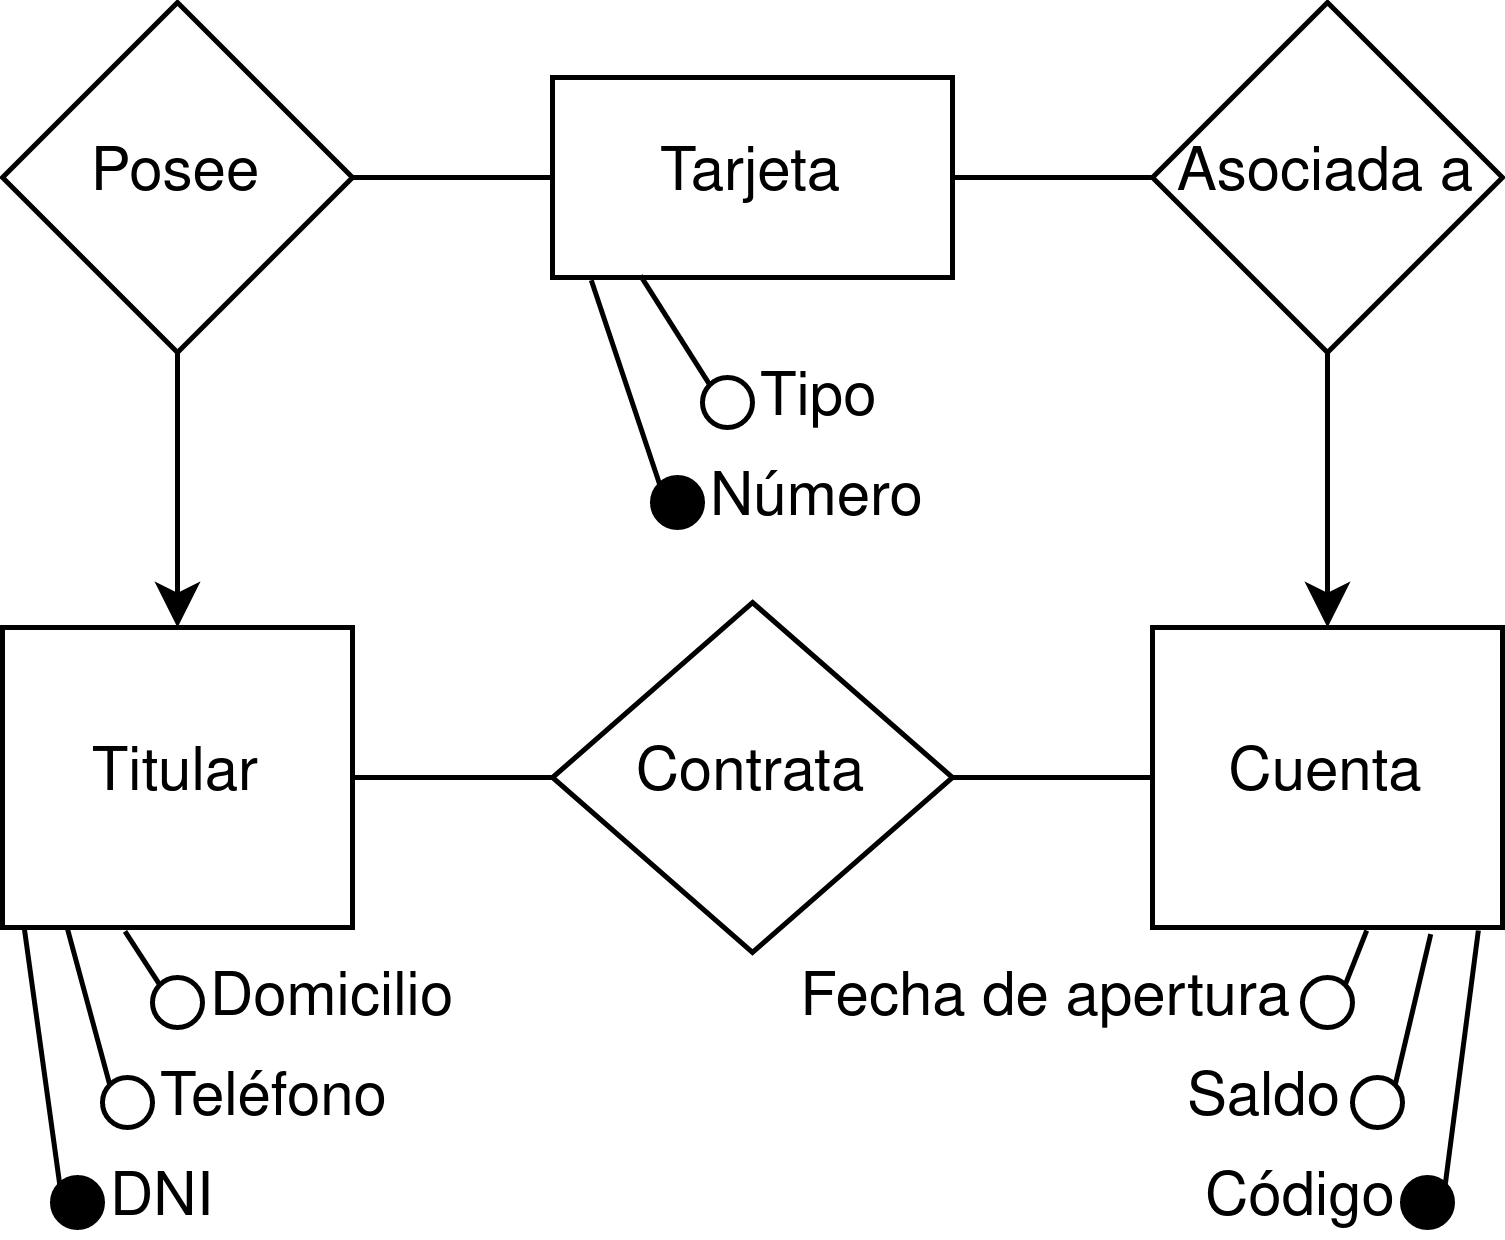
\includegraphics[scale=0.2]{P1Ej1.png}
\end{center}

\section{}\label{ej1-2}

\subsubsection{Enunciado}

En una biblioteca se maneja información acerca de libros, autores, temas, préstamos y usuarios, con los atributos habituales para cada uno.
Las siguientes restricciones semánticas han de cumplirse:

\begin{itemize}
	\item Cada libro puede estar escrito por más de un autor.
	\item Un autor puede escribir más de un libro.
	\item Cada libro puede tratar más de un tema.
	\item Hay muchos libros de cada tema.
	\item La unidad de préstamo es el día.
	\item Cada usuario no puede tener prestado más de un libro simultáneamente (el mismo día).
	\item No existe más que un ejemplar de cada libro.
\end{itemize}

Realizar el diagrama E/R.

\subsubsection{Solución}

\begin{center}
	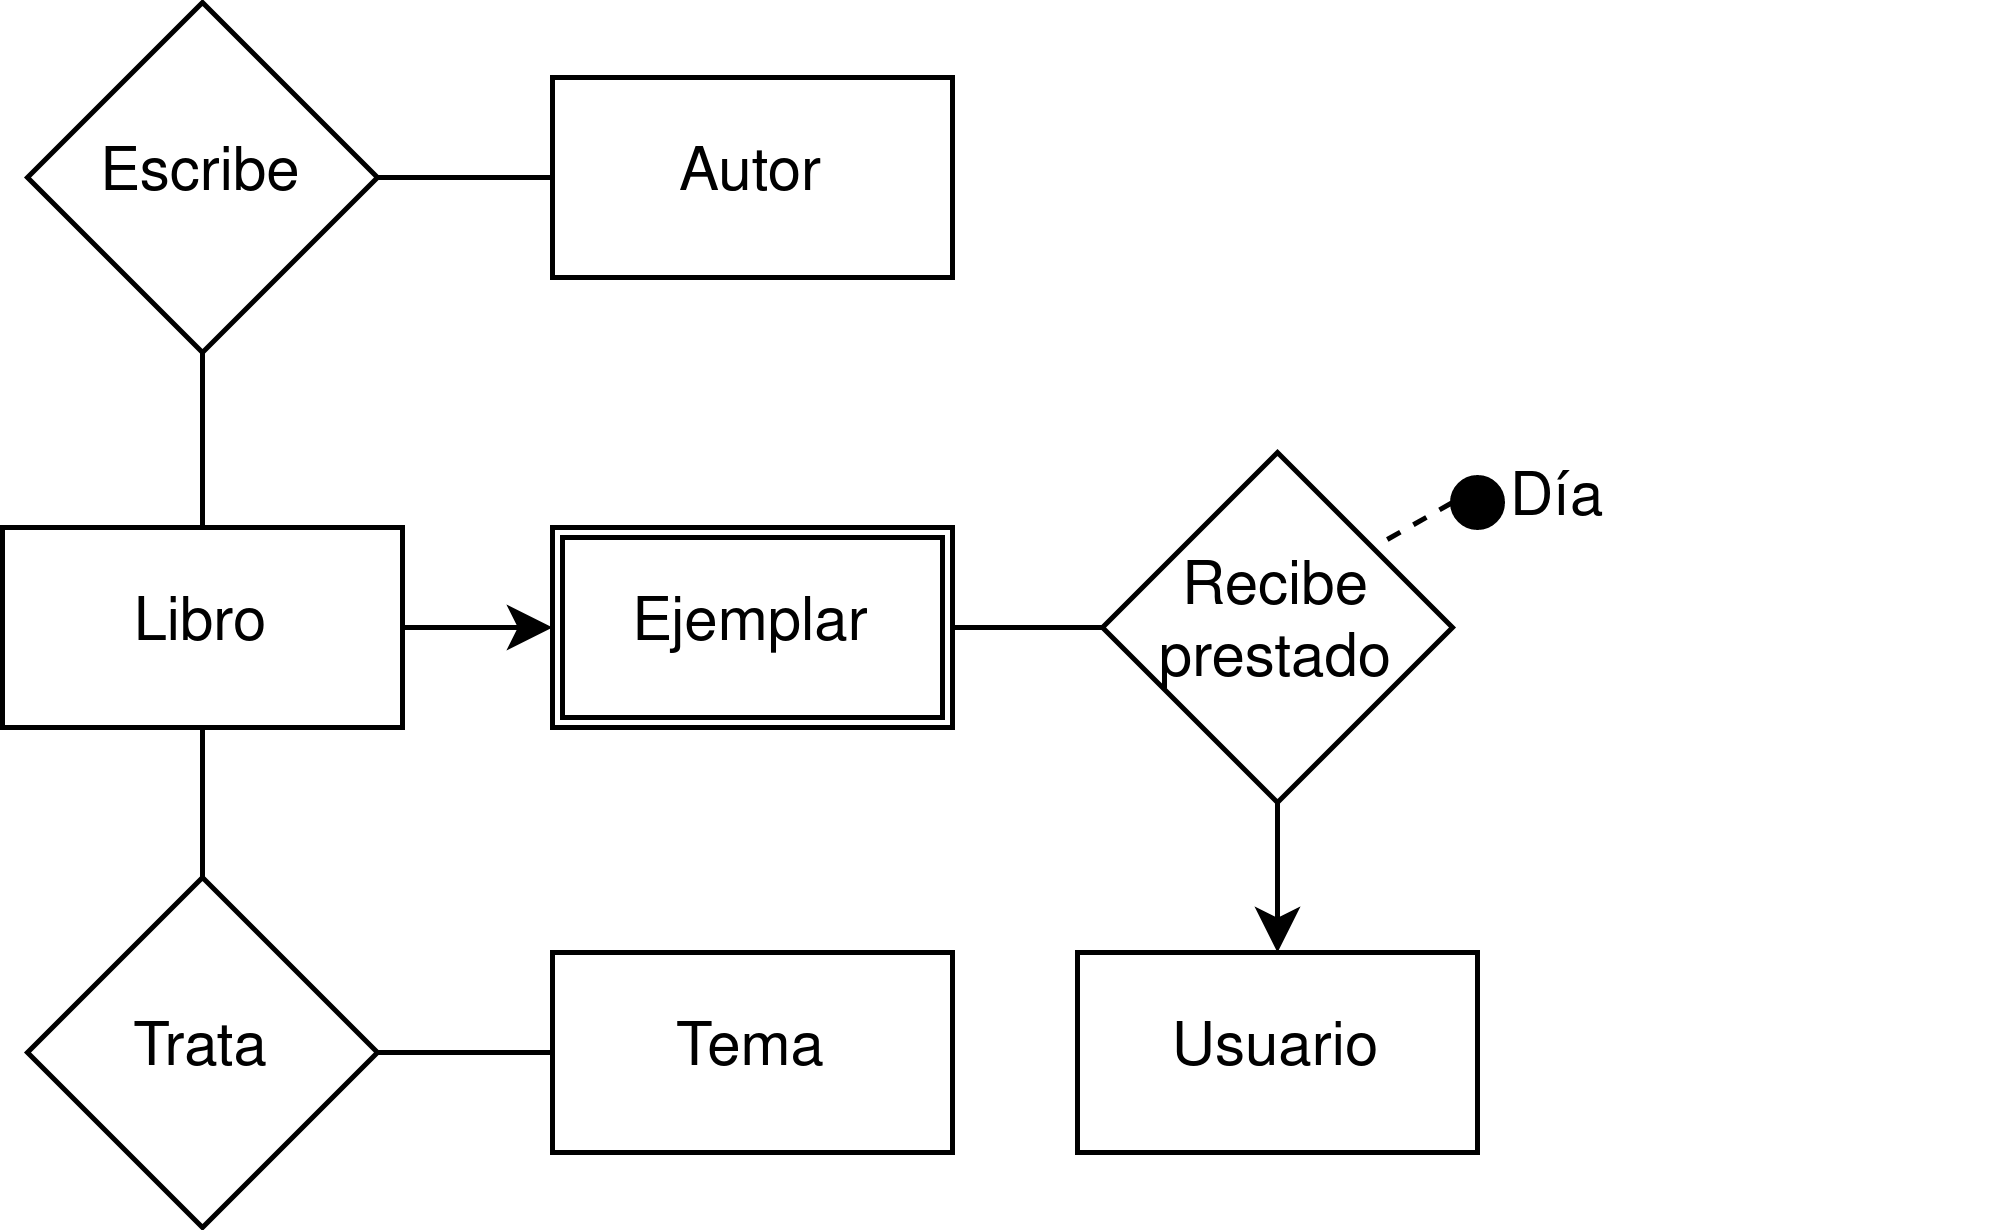
\includegraphics[scale=0.25]{P1Ej2.png}
\end{center}

\setcounter{section}{16}

\section{}\label{ej1-17}

\subsubsection{Enunciado}

Suponemos un sistema de redes sociales (por ejemplo, tipo Facebook):

\begin{itemize}
	\item Un usuario (identificado por su nombre) puede tener varias cuentas (identificadas por código y de las que interesa la fecha de creación y la clave de la cuenta), pero una cuenta sólo puede pertenecer a un usuario.
	\item Existen  varias  apps  (cada  una  identificada  por código),  de las  que nos  interesan especialmente chats (de los que nos interesa el nombre) y wikis (de las que nos interesan título).
	\item Existen recursos, identificados por un código. Hay 3 tipos de recursos: Mensajes de texto (de los que interesa el texto), enlaces a web (de los que interesa la URL) y multimedia (de los que interesa tipo y contenido).
	\item Una cuenta sólo puede acceder a una única app en una fecha y hora concretas (dicho de otro modo: No se permite acceder a dos apps a la vez desde la misma cuenta).
	\item Una cuenta puede compartir un recurso en una o varias apps en una fecha y hora concretas, aunque puede haber varias cuentas publicando recursos (sólo un recurso por cuenta) en la misma app en las mismas fechas y horas.
\end{itemize}

\subsubsection{Solución}

Diagrama E/R\@:

\begin{center}
	\includegraphics[scale=0.055]{P1Ej17}
\end{center}

Paso a tablas:

\begin{center}
	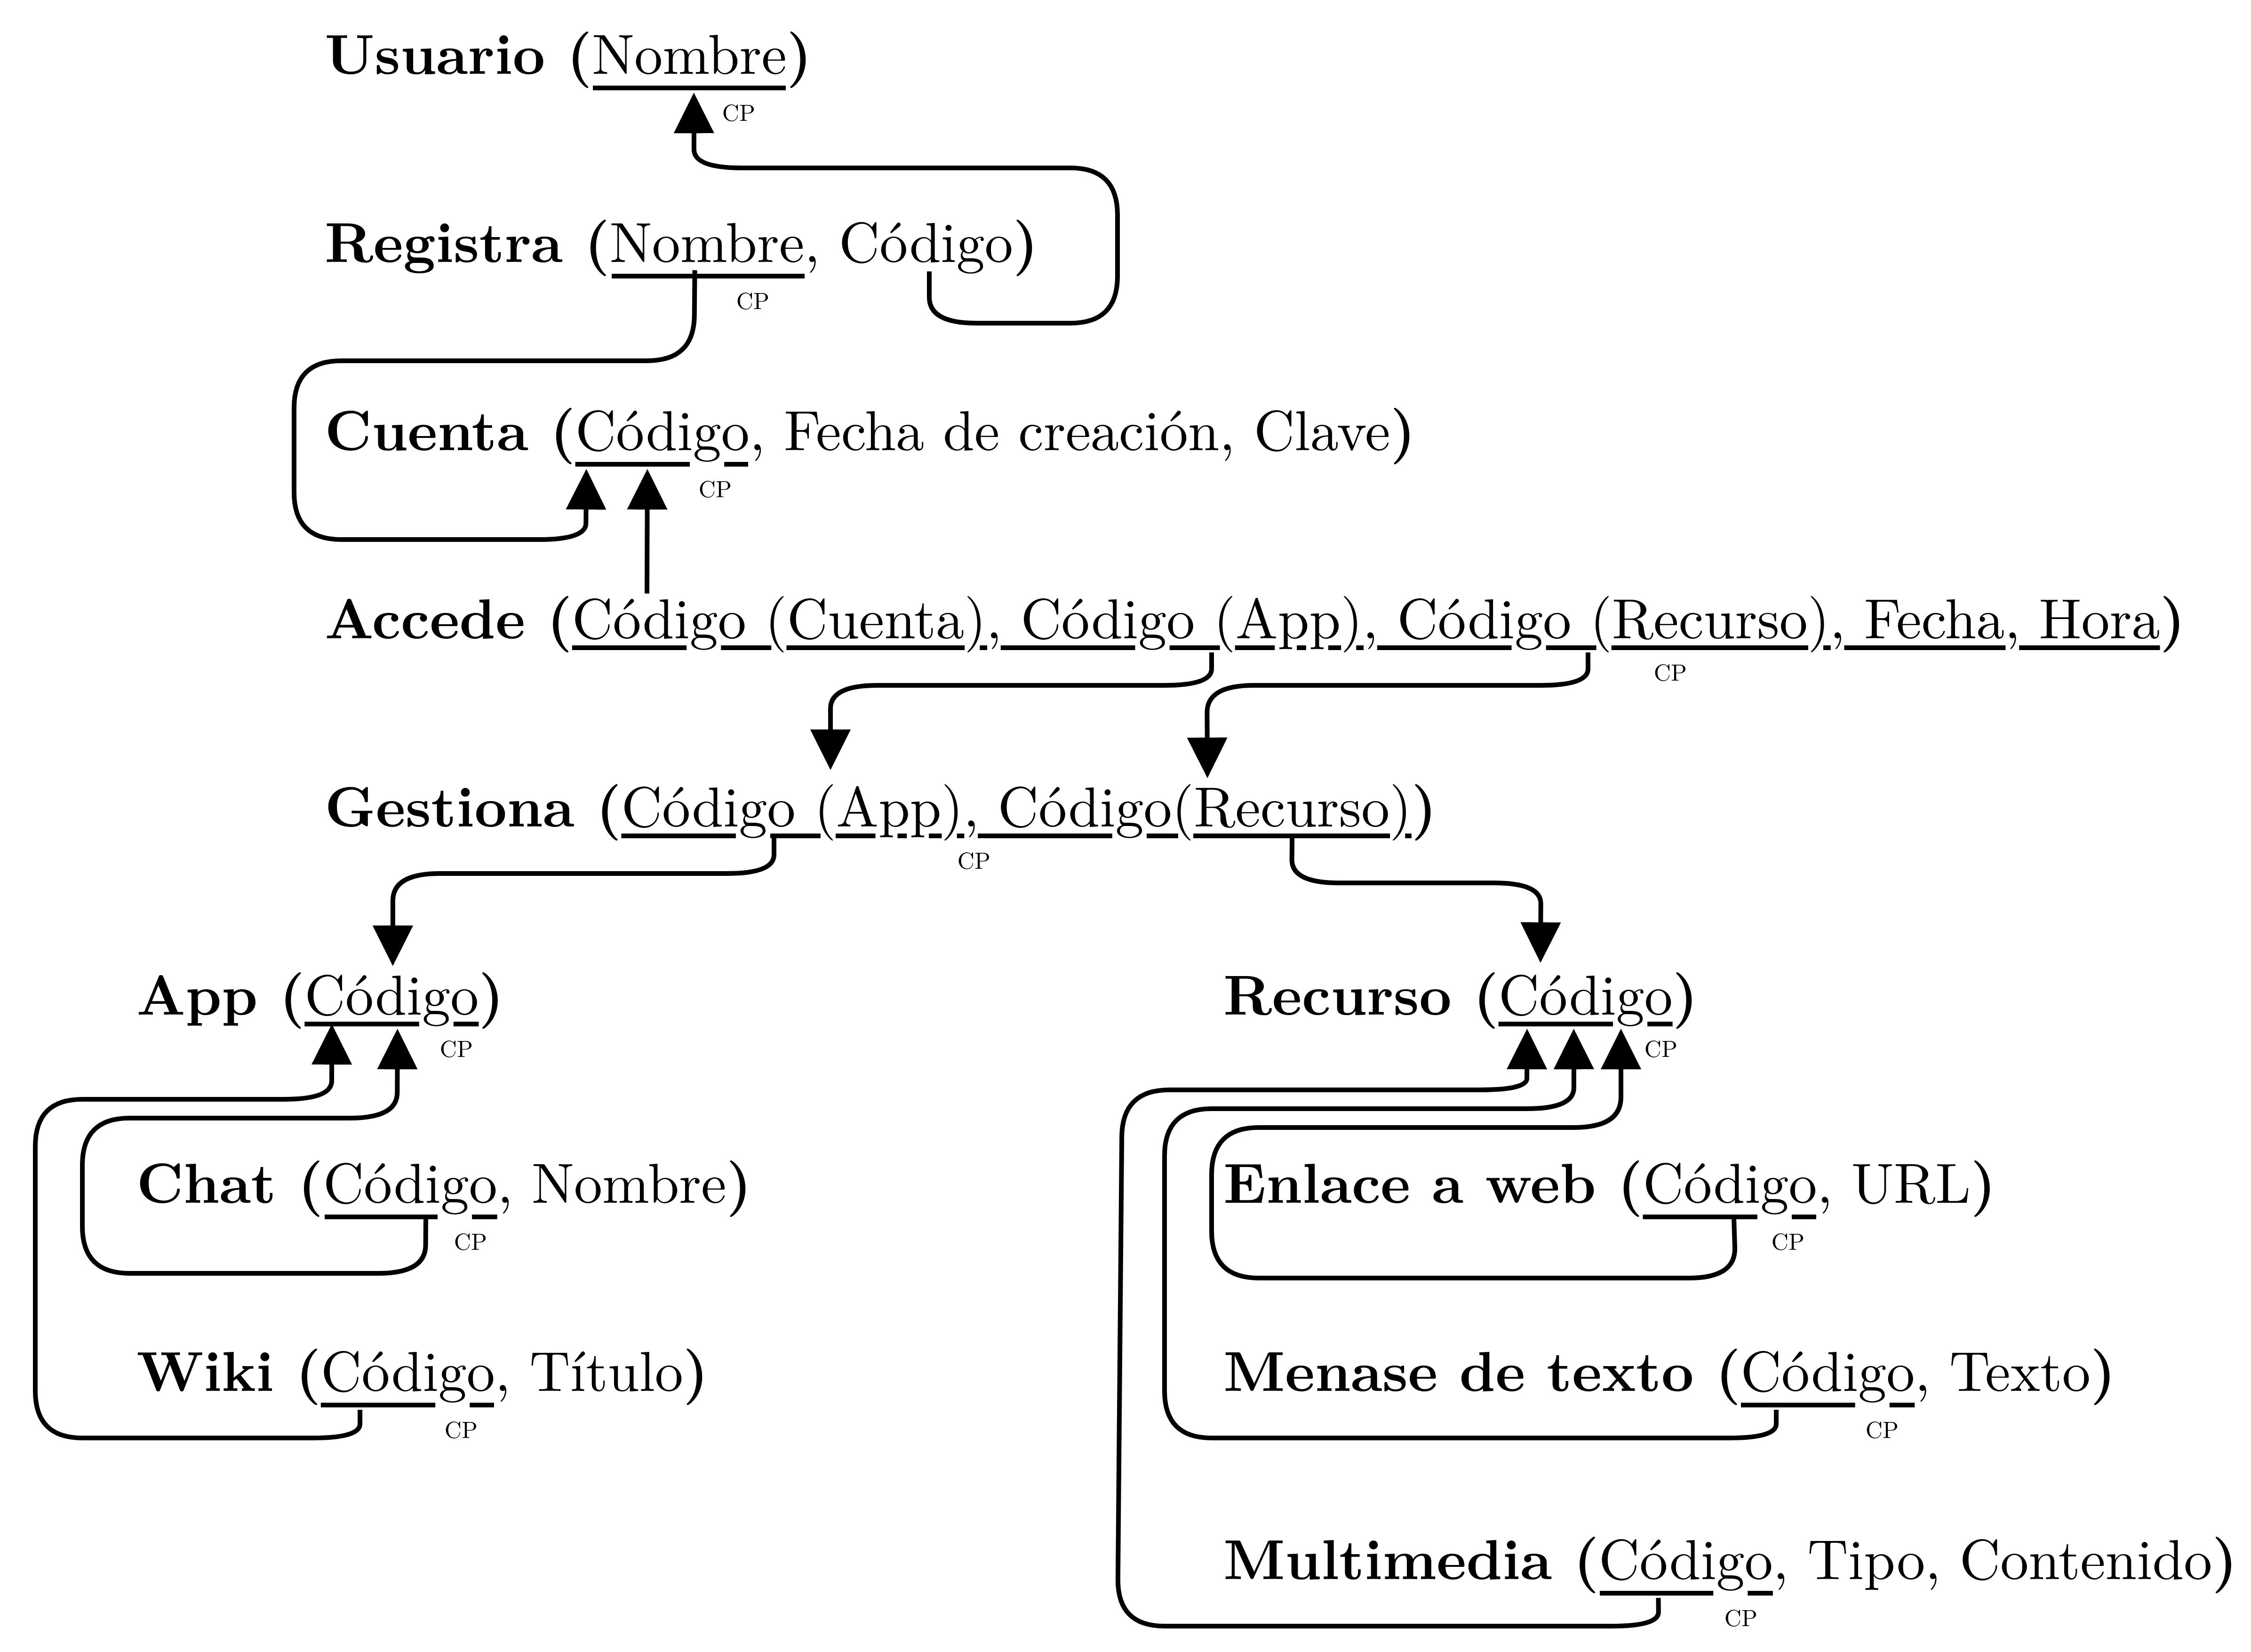
\includegraphics[scale=0.055]{P1Ej17-Tablas}
\end{center}

Fusión de tablas:

\begin{center}
	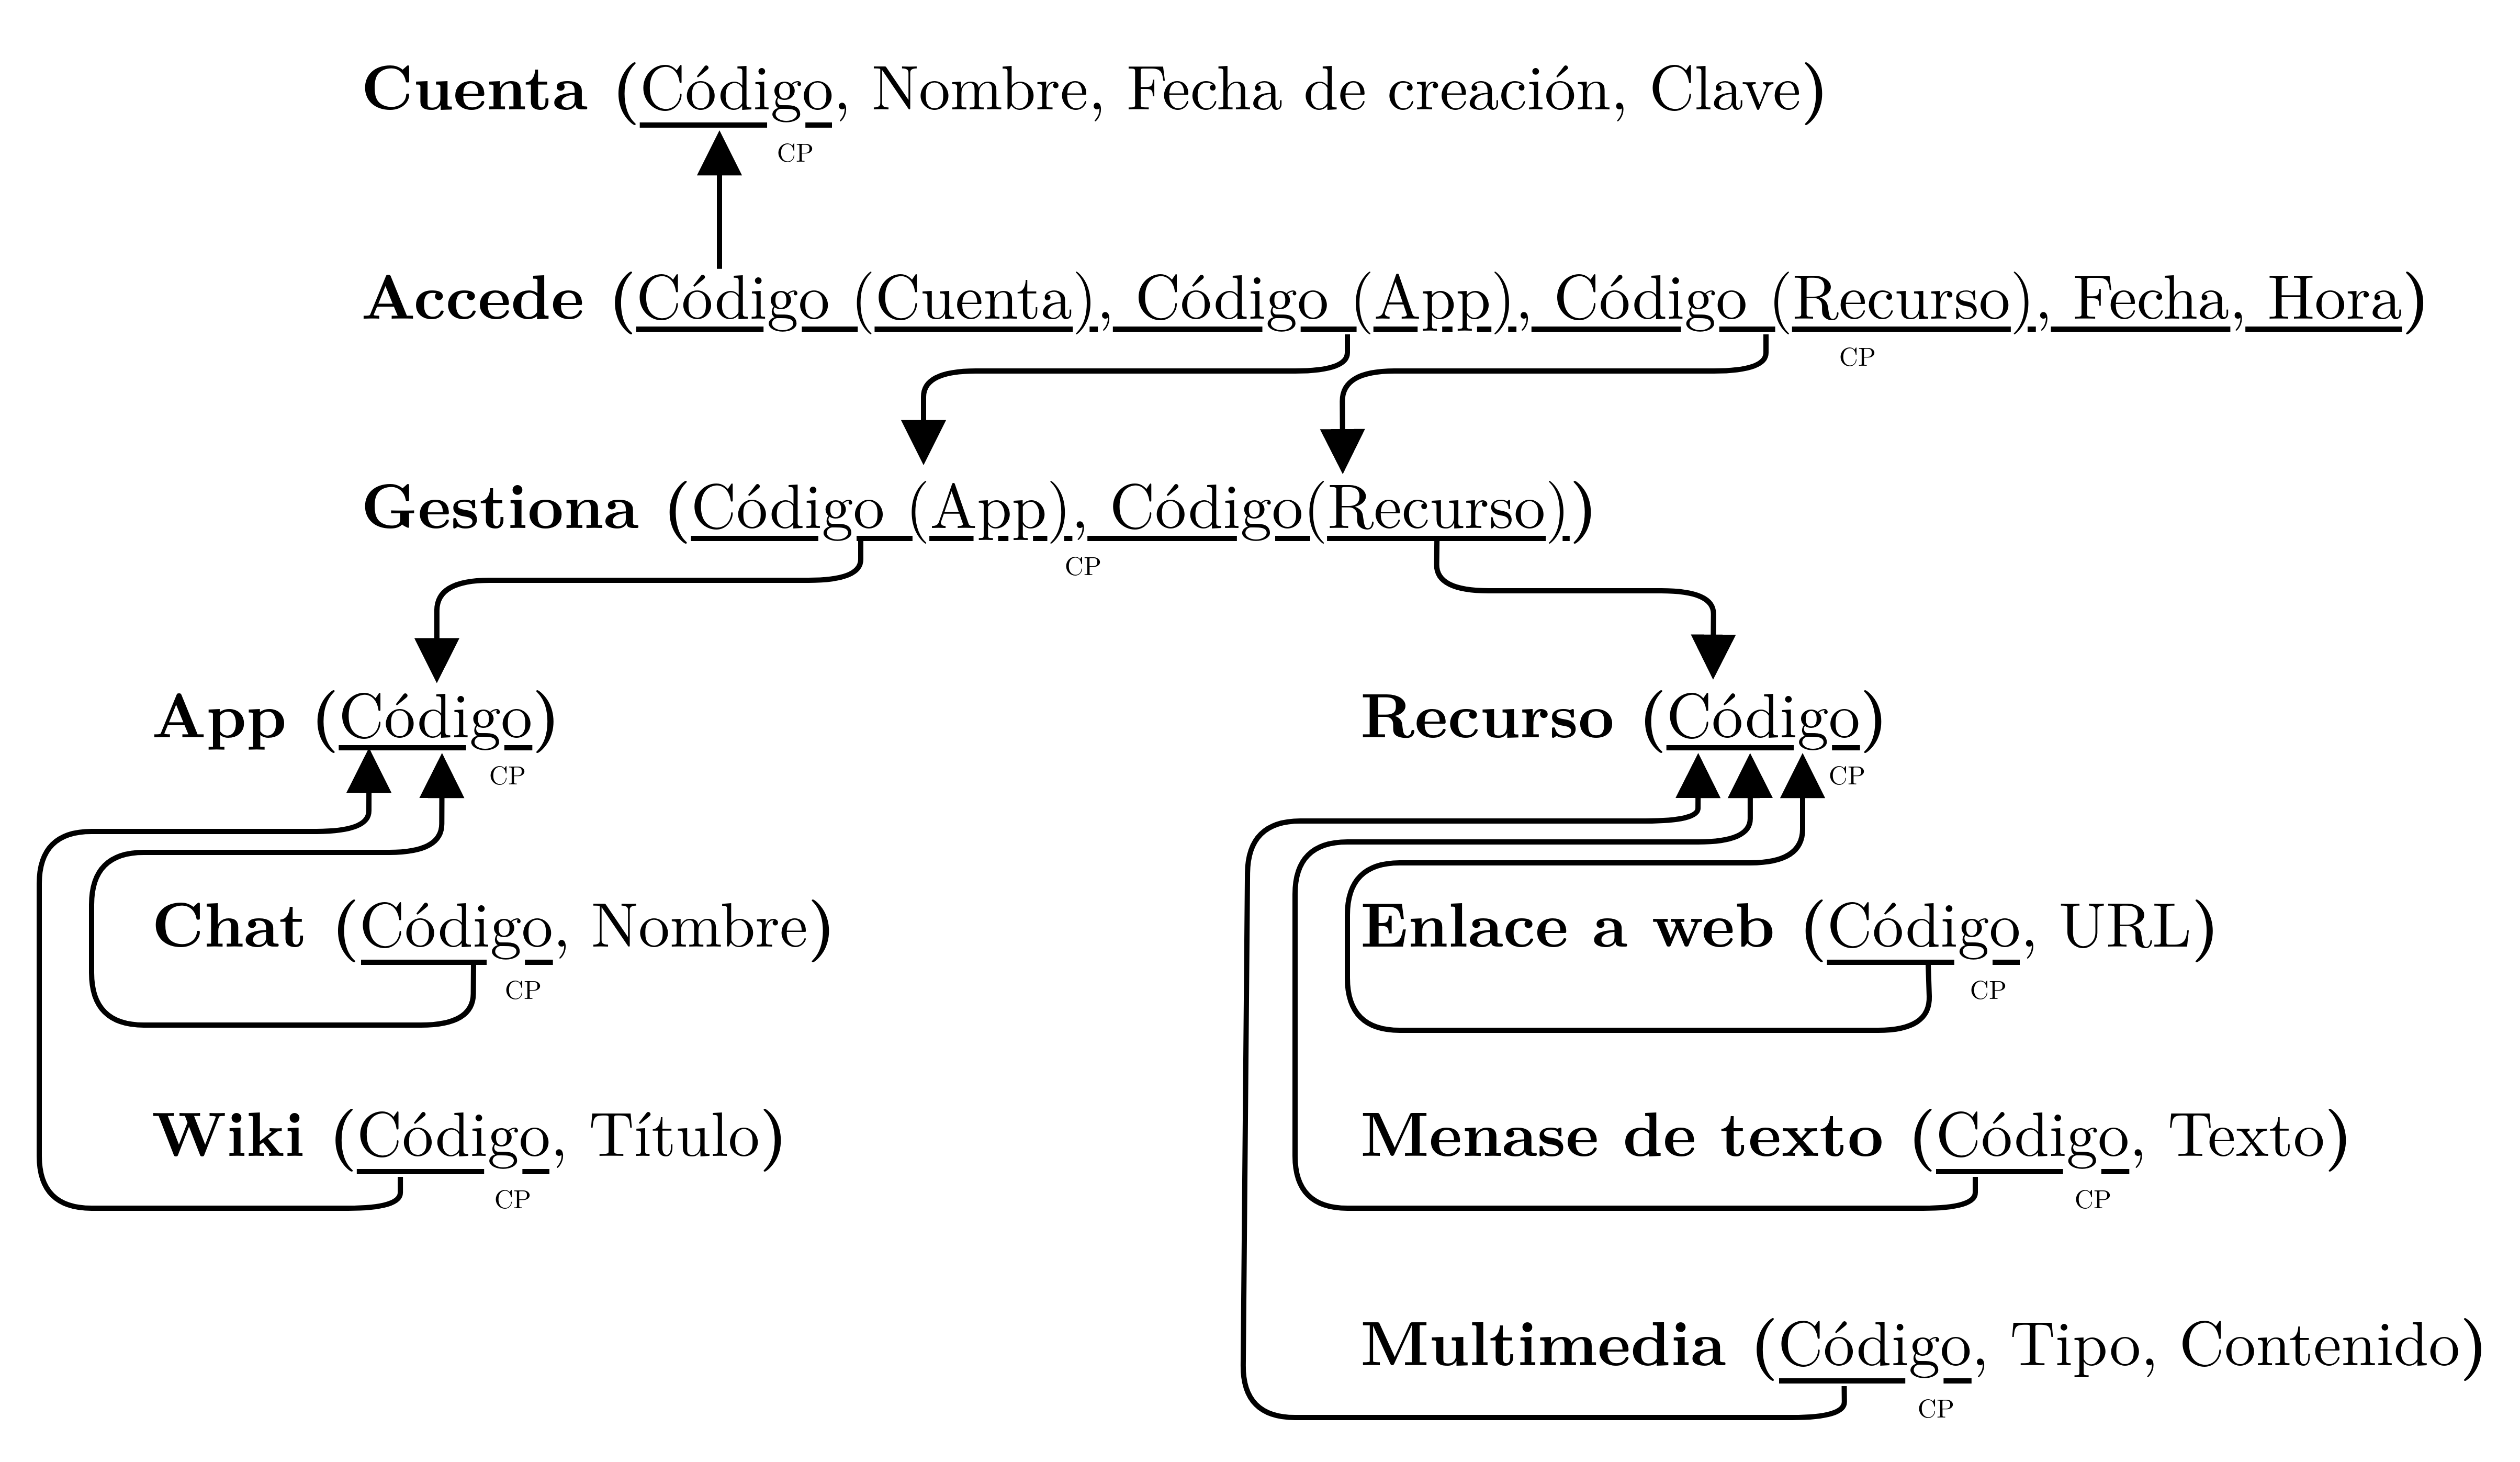
\includegraphics[scale=0.055]{P1Ej17-Fusion}
\end{center}

\aqsec{\S}

\pagebreak

\section{Entrega 21 de marzo}

En el calendario de Prado, la entrega del 21 de marzo se muestra con esta fecha límite.
Sin embargo, al estar programada para cerrarse a las $00:00$, la fecha de entrega final resulta ser el día anterior.
Debido a esto, incluyo el ejercicio de esta entrega en este documento, ya que había programado mi horario de trabajo autónomo para cumplir con la fecha de entrega que muestra Prado.

\subsubsection{Enunciado}

Se trata de organizar los datos de los pedidos realizados por Internet a una tienda on-line.
Los datos y restricciones a considerar son:

\begin{itemize}
	\item Los usuarios deben registrarse mediante un correo electrónico, que debe identificarlos, y la clave de acceso. Además, deben proporcionar su nombre y apellidos. 
	\item Un usuario puede registrar varias direcciones de envío. Cada dirección se identificará mediante una clave y estará descrita por calle, número, piso, letra, código postal y ciudad. Cada dirección estará vinculada a un único usuario.
	\item La tienda admite dos métodos de pago: Tarjetas y Cheques regalo. Ambos se identifican por un número único. De las tarjetas hay que registrar el tipo (Visa, Mastercard, etc) y la fecha de vencimiento (mes/año). De los cheques regalo hay que registrar el importe disponible.
	\item Un cheque regalo está vinculado a una tarjeta concreta, pero la tarjeta puede tener vinculados varios cheques regalo.
	\item Cada método de pago está vinculado a un único usuario. Un usuario puede tener asociados varios métodos de pago.
	\item La tienda dispone de un catálogo de artículos que van identificados mediante un código de referencia; además se dispone de la descripción y del precio unitario del artículo.
	\item Cada pedido se identifica por un código y se debe registrar el total a pagar, la fecha de pedido, la de envío y la de entrega.
	\item Cada pedido puede incluir varias unidades de varios artículos. Un artículo puede aparecer en varios pedidos.
	\item Todo pedido se envía a una de las direcciones registradas. A una dirección se pueden enviar varios pedidos.
	\item Cada pedido lo realiza un usuario cargándose a uno sólo de sus métodos de pago. Un método de pago de un usuario se puede usar en varios pedidos.
\end{itemize}

¿El esquema relacional obtenido impide que un cheque se pueda cargar a otro cheque (en lugar de a una tarjeta)?.

\pagebreak

\subsubsection{Solución}

Diagrama E/R\@:

\begin{center}
	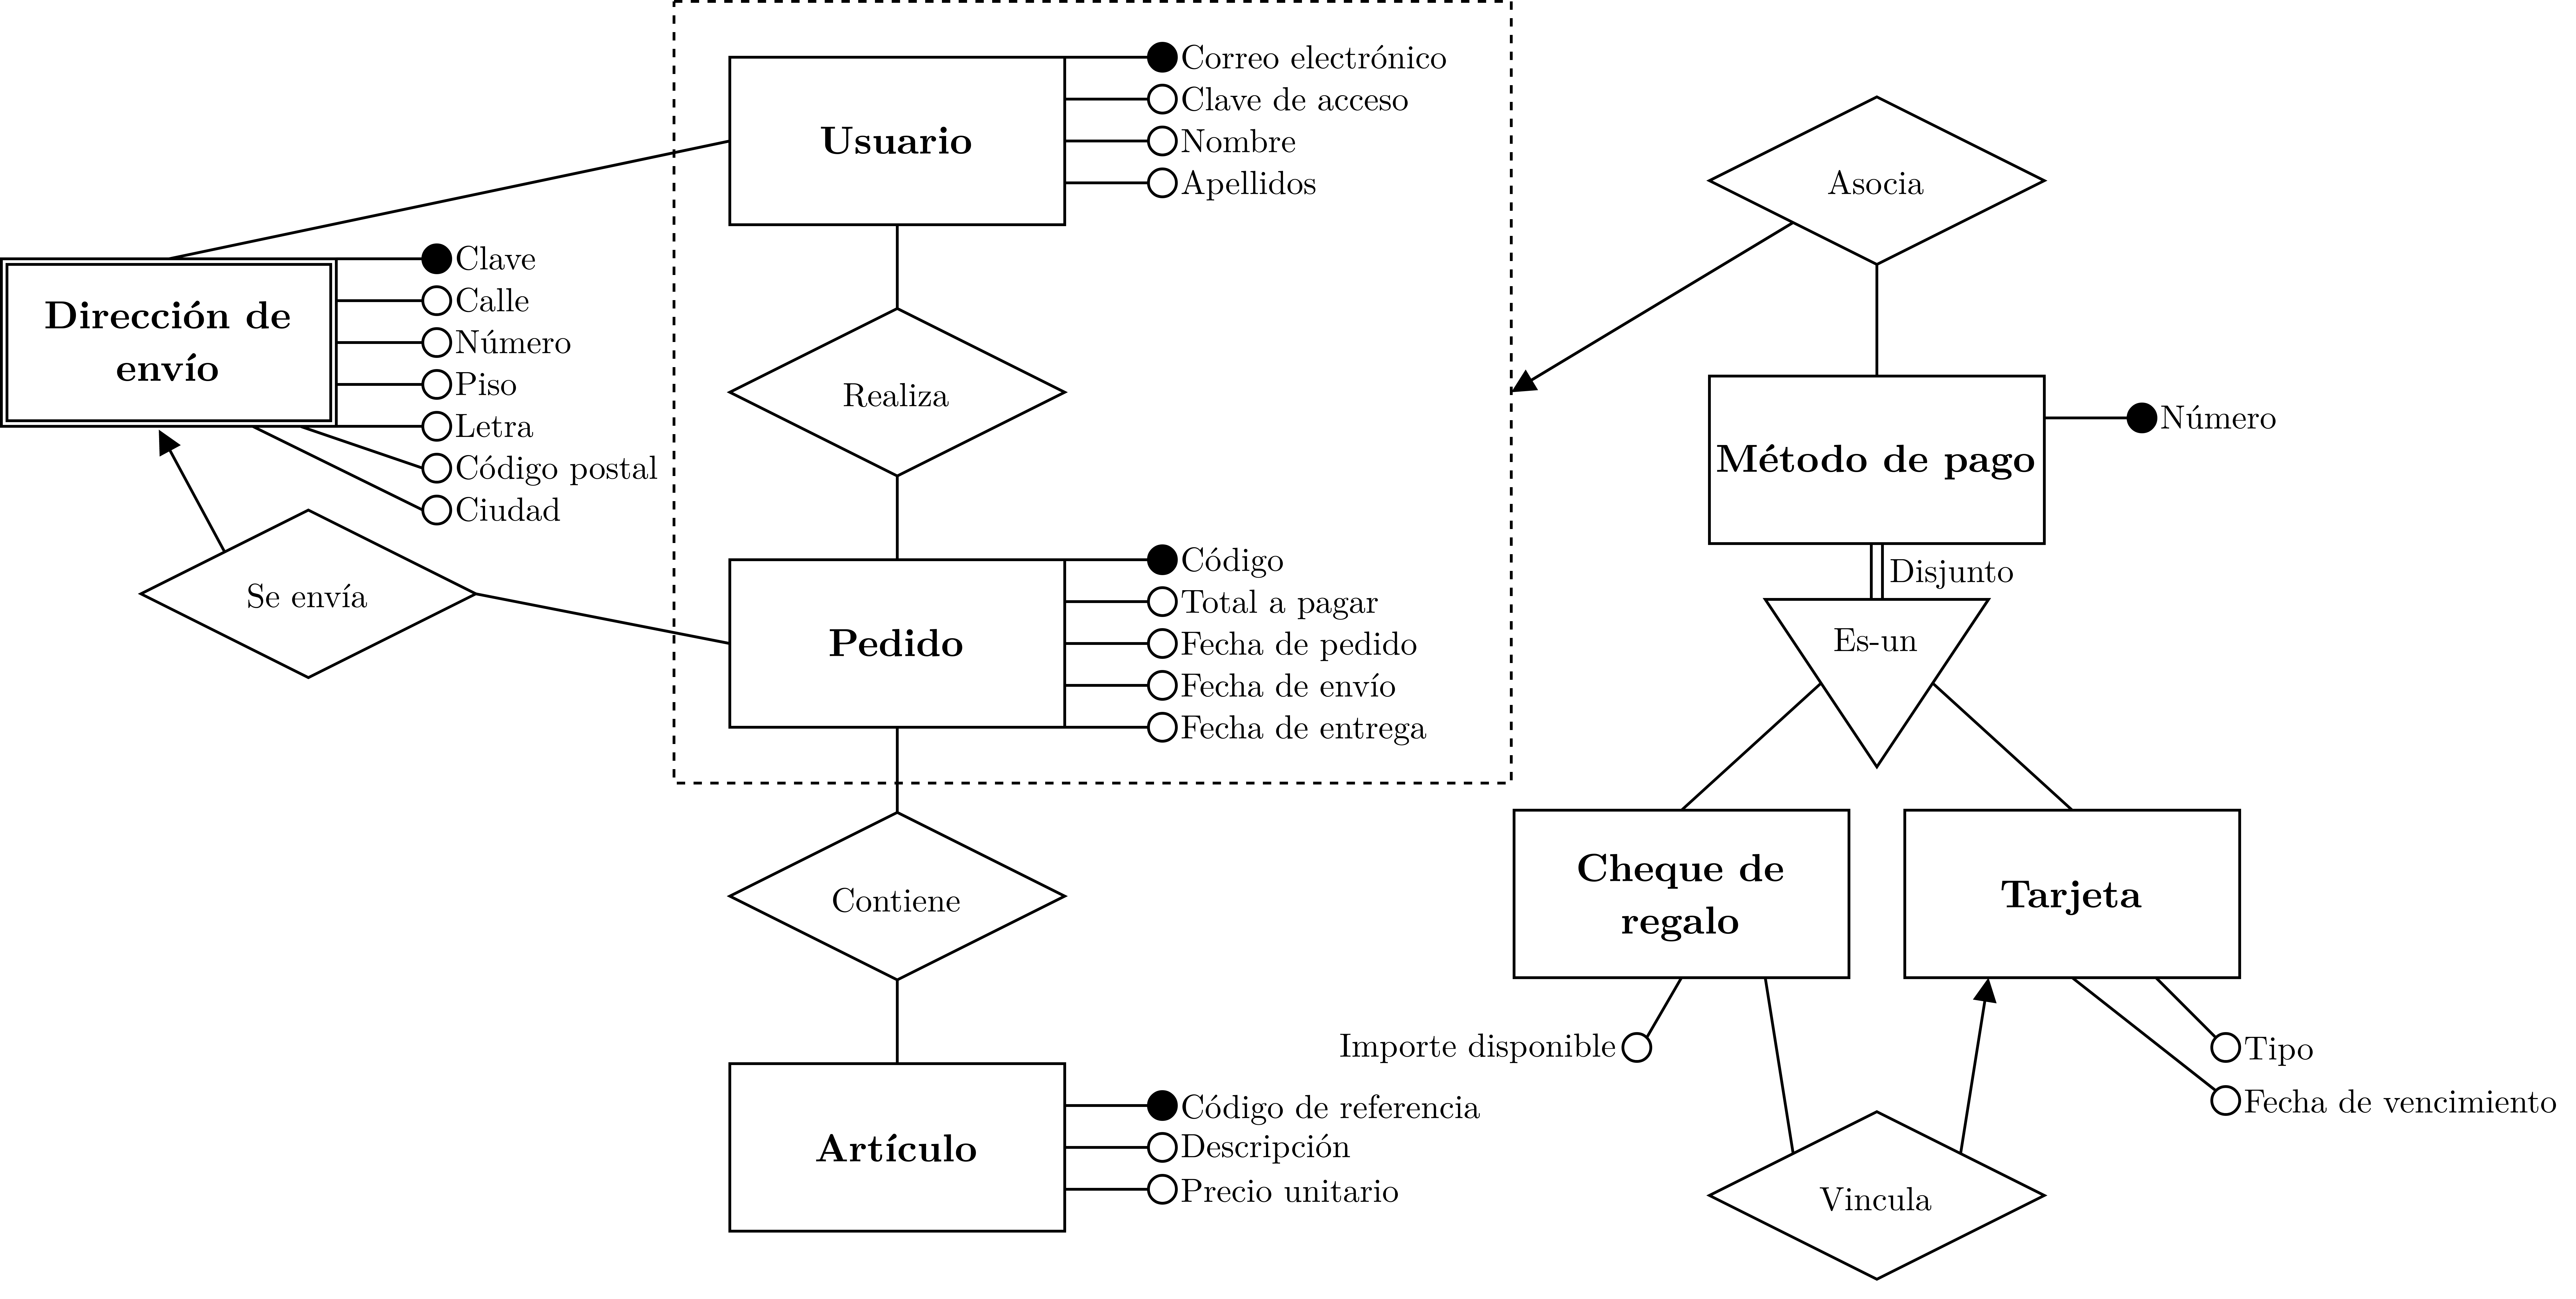
\includegraphics[scale=0.055]{Entrega}
\end{center}

Paso a tablas:

\begin{center}
	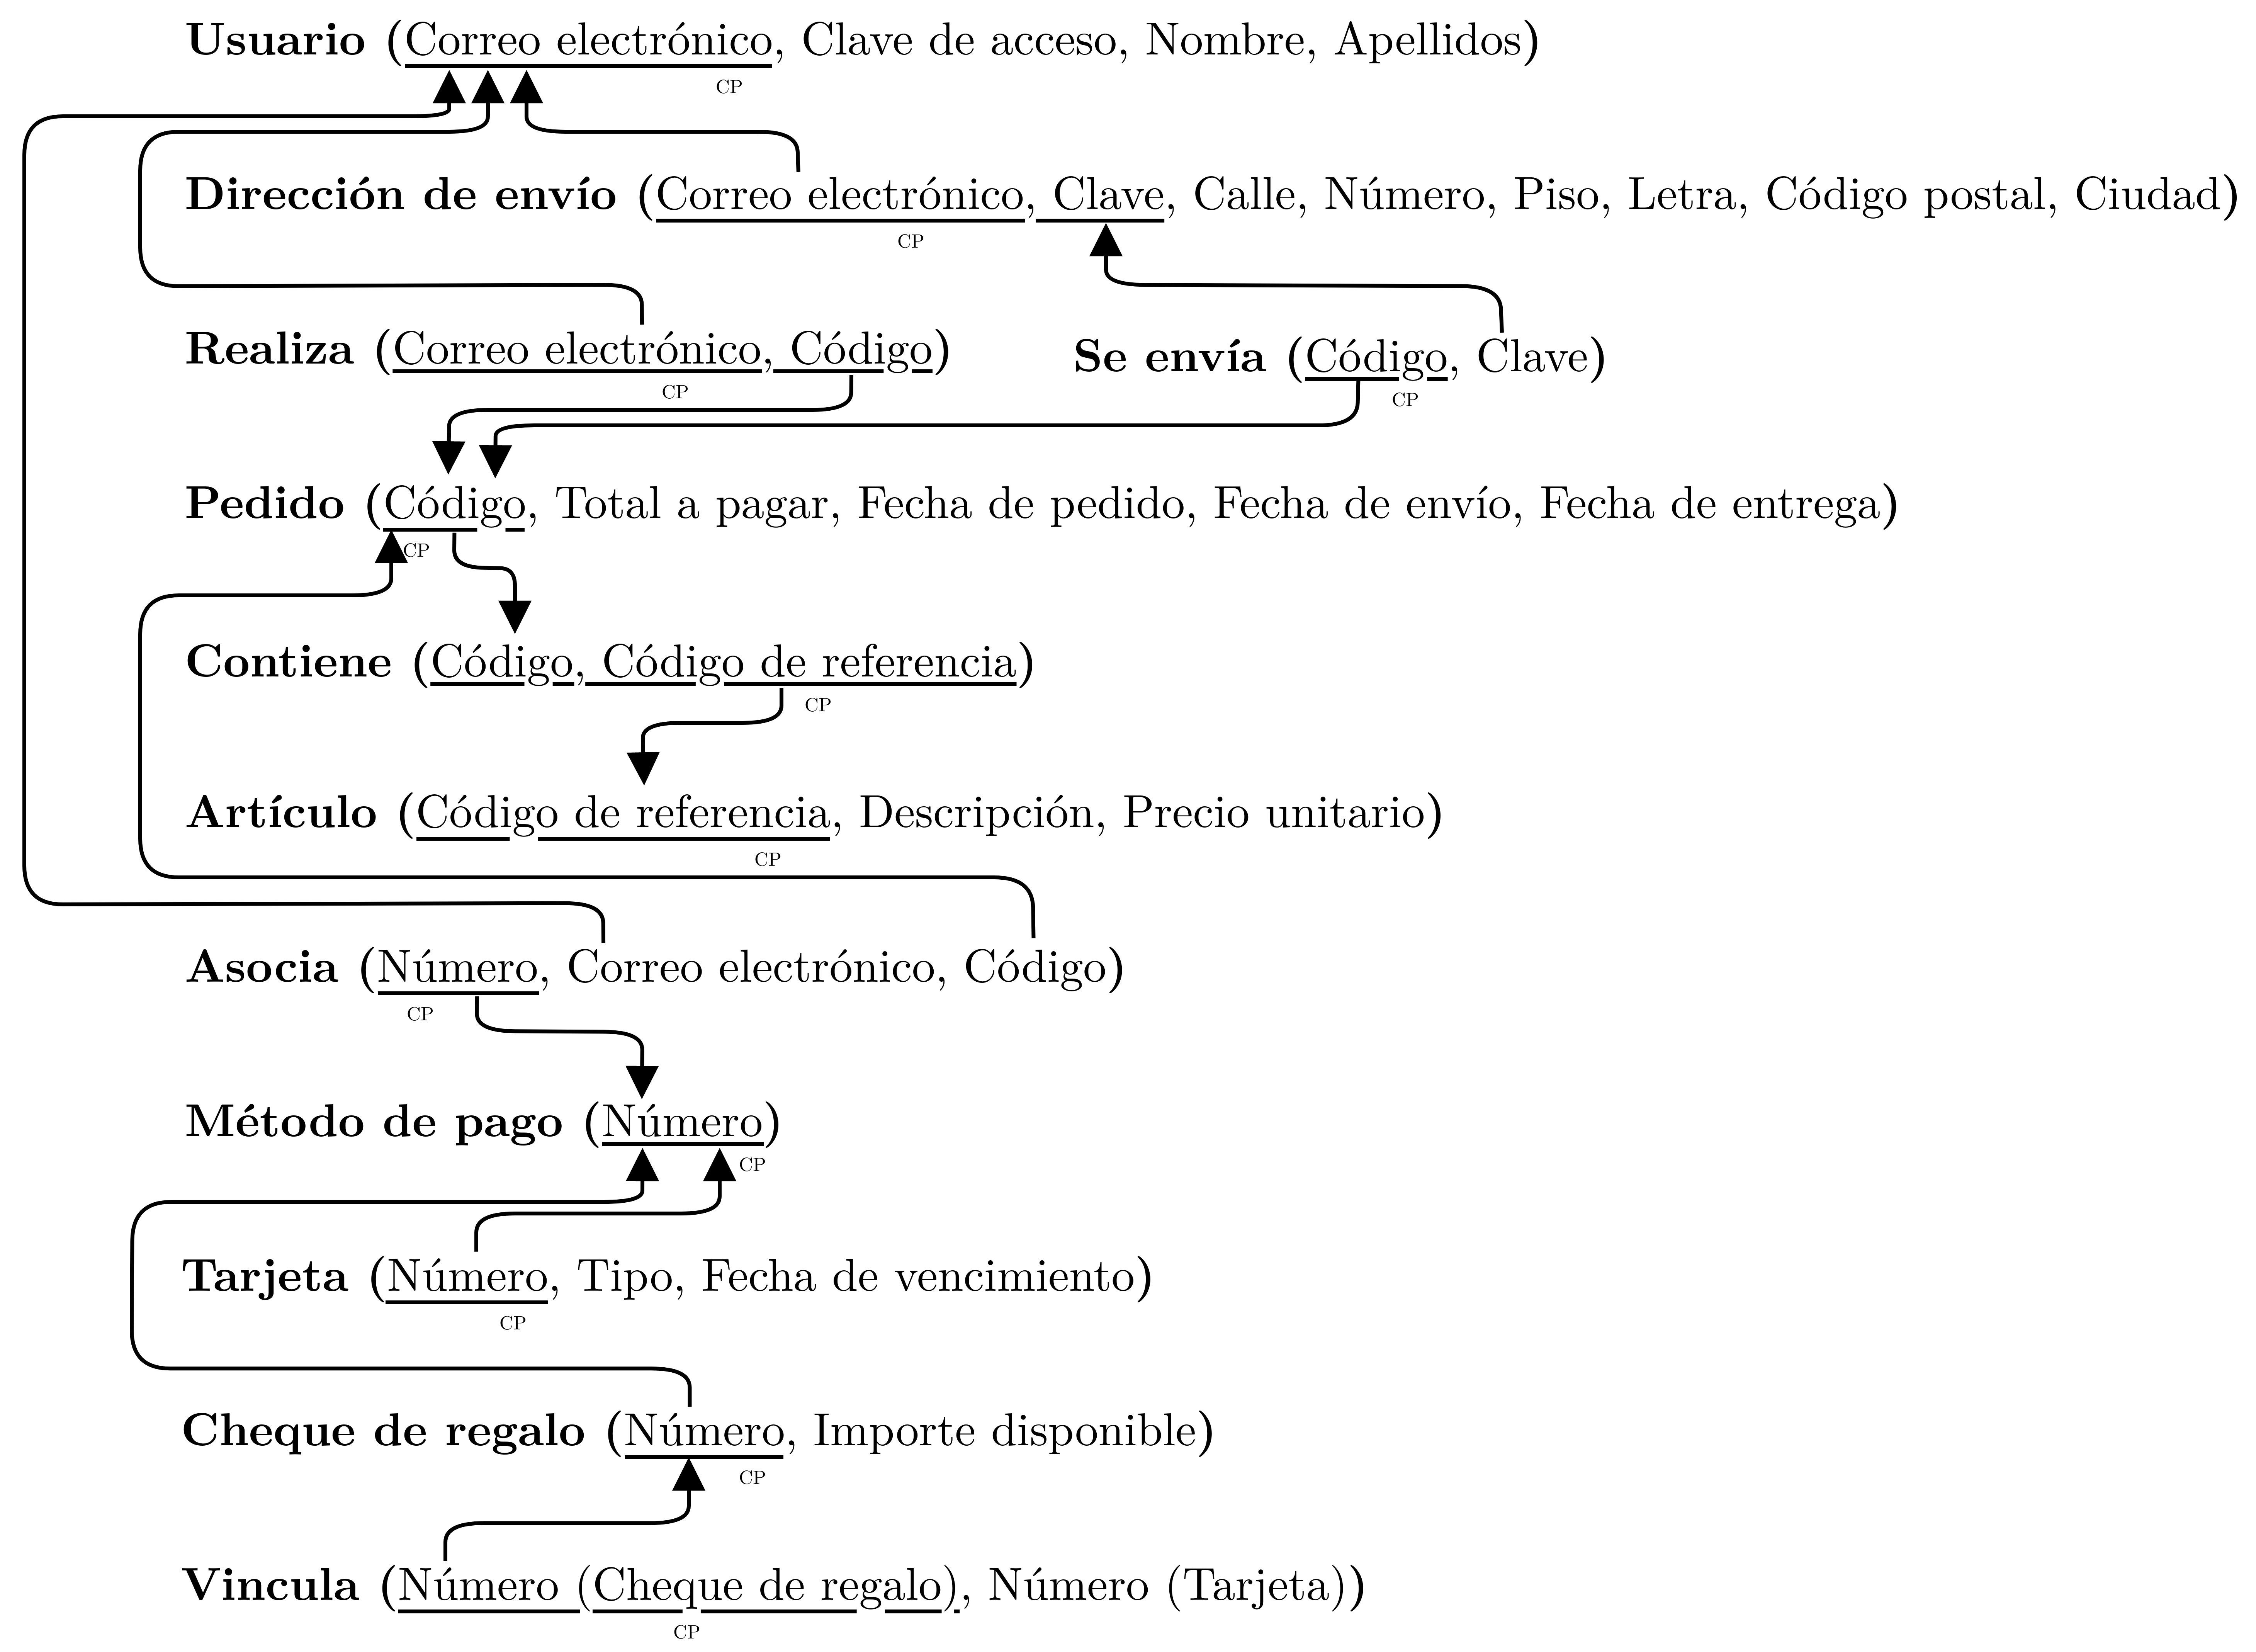
\includegraphics[scale=0.055]{Entrega-Tablas}
\end{center}

Fusión de tablas:

Dado este esquema no resulta viable realizar una fusión de tablas, ya que no hay entidades que puedan fusionarse sin perder información (como las direcciones de envío y los pedidos) o romper relaciones de herencia.

Dado que la relación de vinculación en entre el cheque y la tarjeta y no recursiva para los cheques y que existe una herencia disjunta entre ambas entidades, este esquema impide que un cheque se aplique a otro.
